% !TeX program = xelatex
\documentclass[12pt,a4paper]{article}
\usepackage{fontspec,tikz}
\usetikzlibrary{arrows.meta}
\IfFontExistsTF{Liberation Serif}{\setmainfont{Liberation Serif}}{\setmainfont{FreeSerif}}
\setmonofont{DejaVu Sans Mono}[Scale=.77]
\usepackage[left=25mm,right=23mm,top=22mm,bottom=22mm,footskip=11mm]{geometry}
\usepackage[table]{xcolor}
\usepackage{graphicx,array,tabularx,booktabs,caption,enumitem,amsmath,titlesec,fancyvrb}
\usepackage[hidelinks,unicode]{hyperref}
\hypersetup{pdftitle={IV-2-13. Бие даалт 2. Banker’s Algorithm},pdfauthor={IV-2-13 баг},bookmarksnumbered=true}
\definecolor{peach}{HTML}{EEEAE5}
\definecolor{linecol}{HTML}{B3ACA4}
\definecolor{ink}{HTML}{252626}
\renewcommand{\figurename}{Зураг}
\renewcommand{\tablename}{Хүснэгт}
\renewcommand{\contentsname}{Агуулга}
\renewcommand{\listfigurename}{Зургийн жагсаалт}
\renewcommand{\listtablename}{Хүснэгтийн жагсаалт}
\captionsetup{hypcap=false,font=normalsize,labelfont=bf,justification=centering,skip=5pt}
\setcounter{tocdepth}{1}
\setlength{\parindent}{5mm}
\setlength{\parskip}{4.5pt plus .5pt}
\setlength{\emergencystretch}{3em}
\titleformat{\section}{\large\bfseries}{\thesection.}{.5em}{}
\titleformat{\subsection}{\normalsize\bfseries}{\thesubsection.}{.5em}{}
\titlespacing*{\section}{0pt}{0pt}{8pt}
\titlespacing*{\subsection}{0pt}{9pt}{2pt}
\setlist[enumerate]{leftmargin=7mm,itemsep=3pt,topsep=2pt,parsep=0pt}
\renewcommand{\arraystretch}{1.22}
\setlength{\tabcolsep}{5.5pt}
\newcolumntype{C}{>{\centering\arraybackslash}X}
\newcolumntype{Y}{>{\raggedright\arraybackslash}X}
\newcolumntype{L}[1]{>{\raggedright\arraybackslash}p{#1}}
\newcommand{\code}[1]{\texttt{\detokenize{#1}}}
\newcommand{\hd}{\rowcolor{peach}\bfseries}
\newcommand{\tbl}[3]{\vspace{2pt}\begingroup\centering\small\renewcommand{\arraystretch}{1.32}\setlength{\tabcolsep}{5pt}\setlength{\heavyrulewidth}{.75pt}\setlength{\lightrulewidth}{.35pt}\arrayrulecolor{linecol}\captionsetup{justification=raggedleft,singlelinecheck=false,font=small,labelfont=bf,skip=6pt}\captionof{table}[#1]{#1}\label{#2}#3\par\endgroup\vspace{3pt}}
\newcommand{\fig}[5]{\begin{center}\includegraphics[width=#1\linewidth,height=#2,keepaspectratio]{images/#3.png}\captionof{figure}[#4]{#4}\label{#5}\end{center}}
\newcommand{\lead}[1]{\par\noindent\textbf{#1}\enspace}
\newcommand{\repo}{https://github.com/jal0115/os-bd1-IV-2-13-bankers-algorithm}
\newcommand{\gitlink}[1]{\href{\repo/commit/#1}{\texttt{#1}}}
\makeatletter
\newcommand{\listofart}[2]{{\large\bfseries #1\par}\vspace{2pt}{\small\setlength{\parskip}{0pt}\@starttoc{#2}}}
\makeatother
\linespread{1.065}
\begin{document}
\begin{titlepage}\centering
{\large\bfseries ШИНЖЛЭХ УХААН, ТЕХНОЛОГИЙН ИХ СУРГУУЛЬ\par}
{\large\bfseries Мэдээлэл, холбооны технологийн сургууль\par}
\vspace{9mm}
\includegraphics[height=28mm]{images/must.png}\par
\vspace{11mm}
{\LARGE\bfseries БИЕ ДААЛТ 2\par}\vspace{2mm}
{\LARGE\bfseries ЭЦСИЙН ТАЙЛАН\par}\vspace{6mm}
{\large Үйлдлийн систем (F.CSM302)\par}
{2026–2027 оны хичээлийн жилийн намрын улирал\par}
\vspace{12mm}
\begin{tabularx}{.94\textwidth}{@{}L{43mm}Y@{}}
\textbf{Ажлын нэр} & \textbf{Banker’s Algorithm}\\
& Нөөц хуваарилалт ба аюулгүй дарааллын дүрслэл\\[4pt]
\textbf{Багийн код} & IV-2-13\\
\textbf{Хичээл заасан багш} & Г.Ганбат /F.CS10/\\[4pt]
\textbf{Гүйцэтгэсэн баг} & У.Анужин \hfill B241940071\\
& Г.Лувсанжал \hfill B242270016\\
& Г.Ганхүү \hfill B210930028\\
& Г.Ганжаргал \hfill B222270701\\
& Б.Лхагвадорж \hfill B231940136\\
& Я.Төгөлдөр \hfill B242270806\\
\end{tabularx}
\vfill Улаанбаатар хот\\2026 он
\end{titlepage}
\setcounter{page}{2}
\begin{center}{\Large\bfseries ХУРААНГУЙ}\end{center}
Банкны алгоритм нь процессын хүссэн нөөцийг олгосны дараа бүх процессыг дуусгах боломжтой дараалал үлдэх эсэхийг шалгадаг. Энэхүү ажлаар алгоритмын шийдвэрийг терминалын команд, вэб хүснэгт, нөөцийн графаар тайлбарладаг БД1-ийн программыг II-4-10 багийн шүүмжид үндэслэн сайжруулав. Шүүмжлэгчид цөмийн тооцоо зөв гарч байгааг баталсан ч «Banker-гүй» горимоос номын жишээ рүү товчоор шилжихэд өмнөх горим хадгалагдаж, татгалзах ёстой хүсэлт олгогдож байгааг илрүүлсэн. Мөн Windows PowerShell дээр зааварт өгсөн командын файлыг уншуулахад алдаа гарсан. БД2-т жишээний өгөгдөл, горимыг хамтад нь ачаалдаг болгож, хүснэгтийн засварыг батлах хүртэл хүсэлт илгээх үйлдлийг түгжив. Терминалын программ командын файлыг шууд уншдаг болж, хоёр бэлэн жишээний өгөгдлийг вэб интерфейс ба автомат тестэд нэг эхээс ашигладаг болов. Дахин туршихад номын жишээнд P1-ийн хүсэлтийг олгож, P4-ийг хүлээлгэн, P0-ийн хүсэлтийг түр олгосны дараа аюулгүй дараалал олдоогүй тул буцаасан. Ингэснээр чөлөөтэй нөөц $(2,3,0)$ хэвээр үлдэж, хэрэглэгчийн харсан үр дүн цөмийн тооцоотой таарсан. Debian орчинд шүүмжийн мөрөөр нэмсэн 11 шалгалтыг оролцуулан нийт 75 автомат тест тэнцэв.
\newpage
\begingroup
\setlength{\parindent}{0pt}\setlength{\parskip}{0pt}
\listofart{Агуулга}{toc}\vspace{12pt}
\listofart{Зургийн жагсаалт}{lof}\vspace{12pt}
\listofart{Хүснэгтийн жагсаалт}{lot}
\endgroup
\newpage
\section{Төслийн тойм}
\subsection{Шийдэх асуудал ба хамрах хүрээ}
Төсөл нь \textit{Operating System Concepts} сурах бичгийн 8-р бүлэгт авч үзсэн~\cite{osc} олон төрөлт нөөцийн хуваарилалтыг загварчилна. Процесс бүр ажлаа дуусгах хүртэл төрөл тус бүрээс дээд тал нь хэдэн нэгж хэрэглэхээ урьдчилан мэдэгдэнэ. Нөөцийн нэгжүүд тухайн төрөл дотроо ижил. Процесс дуусахад эзэмшиж байсан нэгжүүд нь бусад процесст ашиглагдах боломжтой болно.

БД1-д Safety шалгалт, нөөц хүсэх ба чөлөөлөх үйлдэл, терминалын интерфейс, графын алхамчилсан тоглуулалтыг хэрэгжүүлсэн. БД2-ын зорилго нь нэг өгөгдлийг CLI болон вэбээр туршихад ижил шийдвэр гарч, хэрэглэгч тэр шийдвэрийн шалтгааныг дэлгэцийн тооноос өөрөө тайлбарлаж чаддаг болоход оршино.

Энэ нь хичээлийн дадлагад хоёр ач холбогдолтой. Оюутан хүсэлтийг олгох эсэхийг эхлээд гараар бодож, дараа нь вектор бүрийн өөрчлөлтийг программын хариутай тулгаж чадна. Мөн ижил хүсэлтийг хамгаалалттай болон хамгаалалтгүй горимоор туршихад гардаг ялгааг ажигласнаар сул нөөц хүрэлцэх нь дангаараа аюулгүй байдлыг батлахгүйг ойлгоно.

\subsection{Номын жишээний эх өгөгдөл}
Таван процесс (P0–P4), гурван төрөл (R0, R1, R2) байна. Хүснэгтийн вектор бүр R0, R1, R2 гэсэн тогтмол дараалалтай. \textit{Max} нь процессын мэдэгдсэн дээд хэрэгцээ, \textit{Allocation} нь одоо эзэмшиж буй хэмжээ. Үлдсэн хэрэгцээг нөөцийн төрөл бүрээр хасаж олно.
\[
 \mathrm{Need}_{ij}=\mathrm{Max}_{ij}-\mathrm{Allocation}_{ij}.
\]
\tbl{Номын жишээний анхны хуваарилалт}{tab:init}{
\begin{tabularx}{\linewidth}{YCCC}\toprule
\hd Процесс & \textbf{Max} & \textbf{Allocation} & \textbf{Need}\\\midrule
P0 & $(7,5,3)$ & $(0,1,0)$ & $(7,4,3)$\\
P1 & $(3,2,2)$ & $(2,0,0)$ & $(1,2,2)$\\
P2 & $(9,0,2)$ & $(3,0,2)$ & $(6,0,0)$\\
P3 & $(2,2,2)$ & $(2,1,1)$ & $(0,1,1)$\\
P4 & $(4,3,3)$ & $(0,0,2)$ & $(4,3,1)$\\\bottomrule
\end{tabularx}}

\lead{Эхний төлвийг шалгах нь.} CLI-д өгдөг $(10,5,7)$ нь нийт нөөц. Хүснэгт~\ref{tab:init}-ийн Allocation баганыг төрөл тус бүрээр нэмбэл $(7,2,5)$ гарна. Иймээс сул нэгж буюу $\mathrm{Available}=(10,5,7)-(7,2,5)=(3,3,2)$. Вэб хүснэгтийн Available нүдэнд энэ үлдэгдлийг шууд оруулна. Жишээлбэл, P1-ийн эхний хэрэгцээ R0 дээр $3-2=1$ байна.
\newpage
\section{Эцсийн архитектур}
\subsection{Нэг цөмийг ашигладаг хоёр интерфейс}
Терминалд \code{RQ 1 1 0 2} гэж бичих, браузерт P1-ийг сонгоод хүсэлтийн гурван нүдэнд 1, 0, 2 гэж оруулах нь цөмд ижил үйлдэл хүргэнэ. CLI текстийг процессын дугаар ба тоон вектор болгоно. Вэб интерфейс эдгээрийг JSON хүсэлтээр илгээж, хариуд ирсэн төлвөөр хүснэгт, граф, аюулгүй дарааллыг дахин зурна.

\tbl{Өгөгдөл дамжих зам ба компонентын үүрэг}{tab:arch}{
\begin{tabularx}{\linewidth}{@{}L{32mm}YY@{}}\toprule
\hd Компонент & \textbf{Хүлээж авдаг өгөгдөл} & \textbf{Гүйцэтгэх ажил}\\\midrule
\code{cli.py} & Нийт нөөц, Max ба Allocation файл, командын мөрүүд. & Available-ийг тооцож цөм үүсгэнэ. Команд бүрийн шийдвэрийг хэвлэнэ.\\\midrule
\code{server.py} & Вэбийн хүсэлт, өгөгдөл ба горим. & Оролтыг шалгаад серверийн түгжээ дотор төлөв шинэчилж, үр дүнг буцаана.\\\midrule
\code{core.py} & Батлагдсан төлөв, процессын дугаар, хүсэх буюу буцаах хэмжээ. & Need, аюулгүй дараалал, алхам бүрийн Work-ийг олно. Аюултай түр олголтыг буцаана.\\\midrule
\code{index.html}, \code{graph.js} & Засварлаж буй хүснэгт, серверээс ирсэн төлөв ба алхмууд. & Хүснэгт, хүсэлт, хариу, түүх болон inline SVG графыг харуулна.\\\midrule
\code{scenarios.json} & 3×2 ба 10×5 жишээний матриц. & Вэб ба автомат тест ижил өгөгдлөөр ижил нөхцөлийг давтана.\\\bottomrule
\end{tabularx}}

\subsection{Засварлаж буй ба батлагдсан төлөв}
Вэб хуудсан дээр Available-ийн R0 нүдийг 3-аас 4 болгоход тоо эхлээд зөвхөн хүснэгтийн засварын хувилбарт орно. Тэр агшинд серверт $(3,3,2)$ үлдсэн хэвээр. Ийм хоёр өөр утга харагдаж болох учраас UI анхааруулга үзүүлж Request, Release болон горимын чагтыг түр түгжинэ. «Шалгах» амжилттай болбол серверийн хариу $(4,3,2)$ болж үйлдлүүд дахин нээгдэнэ.

Номын жишээг ачаалах товч, бэлэн жишээ сонгох цэс хоёр \code{loadPreset()} функцийг ашиглана. Тус функц жишээний өгөгдөлтэй хамт \code{enforce} горимыг дамжуулна. Ингэснээр «Номын жишээ» гэсэн сонголтод Safety шалгалт асаж, хүсэлтийн талбарууд тэглэгдэнэ. Banker-гүй туршилтыг үргэлжлүүлэх бол тухайн жишээг тусад нь сонгоно.
\lead{P1-ийн хүсэлтээр мөрдөх нь.} Вэбээс \code{/api/request} руу процесс 1, хүсэлт $(1,0,2)$ ирэхэд серверийн \code{request()} цөмийн шийдвэрийг авна. Хариуны \code{request_result} хэсэгт «олгосон» эсэх, \code{state} хэсэгт олголтын дараах хуваарилалт ба аюулгүй дараалал ирнэ. Дэлгэцийн мэдэгдэл эхнийхийг, хүснэгт ба граф хоёр дахь хэсгийг уншдаг. Иймээс зөвшөөрөгдөөгүй хүсэлтэд улаан мэдэгдэл гарсан ч аюулгүй төлвийн тэмдэг ногоон хэвээр байж болно.
\newpage

\section{Туршилт ба дүрслэл}
\subsection{Safety шалгалтыг гараар давтах нь}
Алгоритм «яг одоо ямар процесс дуусаж чадах вэ?» гэсэн асуултаар эхэлнэ. \textit{Work} нь шалгалтын явцад сул гэж тооцох нөөцийн түр хуулбар бөгөөд эхний утга нь Available. Дуусаагүй процессын Need векторын бүх элемент Work-ийн харгалзах элементээс ихгүй бол уг процесс ажлаа дуусгаж чадна. Тэр процессын одоо эзэмшиж байгаа Allocation-ийг Work-д нэмж, дараагийн процессыг сонгоно.

Жишээний эхэнд P0-д R0-оос 7 хэрэгтэй ч Work-д 3 байна. P1-д шаардлагатай $(1,2,2)$ нь $(3,3,2)$-т багтана. P1-ийг дууссан гэж үзвэл анх эзэмшиж байсан $(2,0,0)$ чөлөөлөгдөж Work $(5,3,2)$ болно. Цөм процессын дугаарыг багаас их рүү шалгаж, дуусгаж болох эхний процессыг сонгодог.

\tbl{Safety шалгалтын таван алхам}{tab:safety}{
\begin{tabularx}{\linewidth}{c c CCCC}\toprule
\hd № & \textbf{Процесс} & \textbf{Work өмнө} & \textbf{Need} & \textbf{Чөлөөлөх} & \textbf{Work дараа}\\\midrule
1 & P1 & $(3,3,2)$ & $(1,2,2)$ & $(2,0,0)$ & $(5,3,2)$\\
2 & P3 & $(5,3,2)$ & $(0,1,1)$ & $(2,1,1)$ & $(7,4,3)$\\
3 & P0 & $(7,4,3)$ & $(7,4,3)$ & $(0,1,0)$ & $(7,5,3)$\\
4 & P2 & $(7,5,3)$ & $(6,0,0)$ & $(3,0,2)$ & $(10,5,5)$\\
5 & P4 & $(10,5,5)$ & $(4,3,1)$ & $(0,0,2)$ & $(10,5,7)$\\\bottomrule
\end{tabularx}}

Гурав дахь мөрөнд P0-ийн хэрэгцээ Work-тэй яг тэнцүү тул процесс дуусаж болно. Тав дахь мөрийн дараа Work нь системийн нийт нөөц $(10,5,7)$-той тэнцсэн. Иймээс P1 → P3 → P0 → P2 → P4 нь аюулгүй дараалал мөн. Бүх процессыг багтаасан нэг дараалал олоход SAFE дүгнэлт хийхэд хангалттай.

\lead{Яагаад Work-д зөвхөн Allocation нэмдэг вэ?} Тухайн процесс үлдсэн Need-ээ Work-оос аваад ажлаа дуусмагц өмнөх Allocation болон шинээр авсан Need хоёуланг буцаана. Work-ийн цэвэр өсөлт нь өмнө эзэмшиж байсан Allocation-тэй тэнцэнэ. Энэ тооцоо зөвхөн боломжит дарааллыг шалгадаг тул графын «Дараах» товчийг дарахад серверийн бодит Available өөрчлөгдөхгүй.
\lead{Дарааллыг хөтчөөр тулгах нь.} Номын жишээн дээр тоглуулагчийг эхэнд нь байрлуулна. Эхний алхмын өмнө Work $(3,3,2)$, дууссан процессын тоо 0 байна. Нэг алхам ахихад P1-ийн эзэмшиж буй R0-ийн хоёр нэгж чөлөөлөгдөж Work-ийн эхний тоо 3-аас 5 болно. Хоёр дахь алхамд P3 нь R0, R1, R2-оос харгалзан 2, 1, 1 нэгж буцаана. Дэлгэцэд $(7,4,3)$ гарвал граф, хүснэгт хоёул ижил тооцоог харуулж байна.
\newpage
\subsection{Нөөц хүсэх шийдвэрийн схем}
Хүсэлт ирэхэд цөм гурван асуултад дарааллаар нь хариулна. Зураг~\ref{fig:decision}-ийг дээрээс доош уншина. Эхний хоёр шалгалт нь тоонуудыг төрөл тус бүрээр харьцуулна. Харин сүүлийн шалгалт түр олголтын дараа бүх процессыг дуусгах боломжийг тооцно. Схемд оролтын урт ба бүхэл тоон утга зөв, Banker-ийн горим асаалттай тохиолдлыг үзүүлэв.

\begin{center}
\begin{tikzpicture}[font=\normalsize,box/.style={draw,align=center,rounded corners=2pt,inner sep=6pt,text width=58mm},resultbox/.style={draw,align=center,inner sep=6pt,text width=45mm},arr/.style={-{Stealth[length=2.4mm]},semithick}]
\node[box] (n) at (0,0) {Хүсэлт үлдсэн хэрэгцээнд\\багтаж байна уу?};
\node[resultbox] (e) at (8,0) {\textbf{error}\\Дээд хэрэгцээ хэтэрсэн};
\node[box] (a) at (0,-2.1) {Сул нөөц хүрэлцэх үү?};
\node[resultbox] (w) at (8,-2.1) {\textbf{wait}\\Сул нэгжийг хүлээнэ};
\node[box] (t) at (0,-4.1) {Нөөцийг түр олгоно};
\node[box] (q) at (0,-6.2) {Аюулгүй дараалал\\олдсон уу?};
\node[resultbox] (u) at (8,-6.2) {\textbf{unsafe}\\Түр олголтыг буцаана};
\node[box] (g) at (0,-8.3) {\textbf{granted}\\Олголтыг батална};
\foreach \x/\y in {n/e,a/w,q/u}{\draw[arr] (\x) -- node[above]{Үгүй} (\y);}
\foreach \x/\y in {n/a,a/t,q/g}{\draw[arr] (\x) -- node[right]{Тийм} (\y);}
\draw[arr] (t) -- (q);
\end{tikzpicture}
\captionof{figure}{Banker идэвхтэй үед хүсэлтийг шийдэх дараалал}\label{fig:decision}
\end{center}

Схемийн баруун талд гарсан гурван хариу өөр шалтгаантай ч батлагдсан төлөвийг хадгална. Эхний хоёр салаанд нөөц хөдлөхгүй. Гурав дахь салаанд нөөц аль хэдийн түр шилжсэн учраас Available болон тухайн процессын Allocation-ийг өмнөх утгад нь сэргээнэ. Дараах туршилтад энэ ялгааг нэг эх төлөвөөс бодож харууллаа.
\newpage
\subsection{Гурван хүсэлтийн шийдвэр ба rollback}
Номын жишээг нэг удаа ачаалаад доорх хүсэлтүүдийг \textbf{дунд нь дахин ачаалахгүйгээр} дараалуулна. Хүсэлт бүр зөвшөөрсөн дээд хэрэгцээнд багтаж байгаа эсэхийг эхэлж шалгана. Дараа нь чөлөөтэй нөөц хүрэлцэх эсэхийг үзнэ. Хоёр нөхцөл биелбэл түр олгосны дараах төлөв дээр Safety алгоритмыг ажиллуулна.

\tbl{Дараалсан хүсэлт бүрийн дараах батлагдсан төлөв}{tab:req}{
\begin{tabularx}{\linewidth}{@{}L{25mm}L{21mm}YL{22mm}@{}}\toprule
\hd Хүсэлт & \textbf{Шийдвэр} & \textbf{Шалтгаан} & \textbf{Available}\\\midrule
P1 $(1,0,2)$ & \code{granted} & Түр олгосны дараа P1-ийн үлдсэн Need $(0,2,0)$-г хангаж чадна. Бүх процесс дуусах дараалал үлдэв. & $(2,3,0)$\\\midrule
P4 $(3,3,0)$ & \code{wait} & P4-ийн хэрэгцээнд багтсан ч R0-оос 3 хүсэхэд 2 сул байна. Түр олголт эхлэхгүй. & $(2,3,0)$\\\midrule
P0 $(0,2,0)$ & \code{unsafe} & Хүссэн R1 хүрэлцэнэ. Түр олгоход бүх процессыг дуусгаж болох дараалал алга болсон тул буцаана. & $(2,3,0)$\\\bottomrule
\end{tabularx}}

\lead{P0 дээр юу буцаасан бэ?} Хүсэлтийн өмнө P0-ийн Allocation $(0,1,0)$, Need $(7,4,3)$. R1-ээс хоёр нэгжийг түр олговол эдгээр нь $(0,3,0)$ ба $(7,2,3)$ болно. Сул нөөц $(2,1,0)$ болон багасна. Ийм Work-оор P0-д R0, P1-д R1, P2-т R0, P3-т R2, P4-т R0 хүрэлцэхгүй. Эхэлж дуусгах процесс ганц ч олдсонгүй.

\tbl{P0-д R1-ээс хоёр нэгж түр олгоод буцаахад}{tab:rollback}{
\begin{tabularx}{\linewidth}{L{40mm}CCC}\toprule
\hd Хэмжигдэхүүн & \textbf{Хүсэхийн өмнө} & \textbf{Түр олгосон} & \textbf{Буцаасны дараа}\\\midrule
Available & $(2,3,0)$ & $(2,1,0)$ & $(2,3,0)$\\
P0-ийн Allocation & $(0,1,0)$ & $(0,3,0)$ & $(0,1,0)$\\
P0-ийн Need & $(7,4,3)$ & $(7,2,3)$ & $(7,4,3)$\\\bottomrule
\end{tabularx}}

Цөм түр олгосон хоёр нэгжийг Available-д буцааж, P0-ийн Allocation-оос хасна. Ингэснээр P0-ийн Need мөн анхны утгаа авна. Дэлгэцэд хүсэлтийн хариу \code{unsafe} гэж гарсан ч батлагдсан системийн төлөв \textbf{SAFE} хэвээр байна. Нэмсэн тест хүсэлтийн өмнөх ба дараах серверийн төлвийг бүхэлд нь тулгадаг.

\lead{Хяналтын туршилт.} «Banker-гүй» жишээг эхнээс нь ачаалаад P1 $(1,0,2)$, P0 $(0,2,0)$ гэж дахин хүснэ. Дээд хэрэгцээ, чөлөөтэй нөөцийн шалгалт хэвээр боловч Safety шалгалтыг алгасдаг тул P0-д энэ удаа хоёр нэгжийг олгож, Available $(2,1,0)$ үлдэнэ. Энэ нь бүх процесс дээд хэрэгцээндээ хүрч дуусах баталгаа алдагдсаныг харуулна. Бодит deadlock үүссэнийг тогтооход процессууд яг одоо юуг хүлээж байгааг мөн мэдэх хэрэгтэй~\cite{osc,coffman}.
\newpage
\subsection{Вэб хүснэгтээс шийдвэрийг унших нь}
Зураг~\ref{fig:book}-т хуудасны хоёр хэсгийг томруулж харуулав. «Номын жишээг оруулах» товч дарсны дараа эхлээд R0, R1, R2-ын Available $(3,3,2)$ болон Banker-ийн чагтыг шалгана. Хүсэх хэмжээг баруун талын гурван нүдэнд оруулна. Зүүн талын Available-ийг соливол туршилтын анхны нөхцөл өөрчлөгдөнө.
\begin{center}
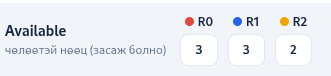
\includegraphics[width=.63\linewidth]{images/free.png}\\[4pt]

\includegraphics[width=.61\linewidth]{images/mode.png}
\captionof{figure}{Номын жишээ ачаалсны дараах хоёр хэсэг. Дээд зурагт сул нөөц, доод зурагт идэвхтэй Banker горим харагдана.}\label{fig:book}
\end{center}

\begin{minipage}[t]{.50\linewidth}\vspace{0pt}
\textbf{Зөвшөөрсөн хэрэгцээнээс хэтэрвэл.}
Номын анхны төлөв дээр P0-ийн R0 хэрэгцээ 7. Хүсэлтийн R0 нүдэнд 99 оруулахад эхний шалгалт дээр шалтгааныг «хүсэлт=99, Need=7» гэж харуулна. Энэ тохиолдолд цөм \code{error} хариу өгнө. Safety шалгалт, түр олголт хоёул алгасагдана.

Харин хүснэгт~\ref{tab:req}-ийн P4 хэрэгцээгээ хэтрүүлээгүй. Зөвхөн тухайн үеийн сул нэгж хүрээгүй тул \code{wait} гэсэн өөр шийдвэр гарсан.
\end{minipage}\hfill
\begin{minipage}[t]{.46\linewidth}\vspace{0pt}\centering
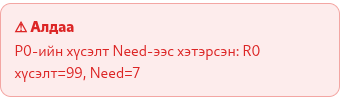
\includegraphics[width=\linewidth,height=72mm,keepaspectratio]{images/error.png}
\captionof{figure}[P0-ийн оролтын алдаа]{P0-ийн $(99,0,0)$ хүсэлтийг шалгасан нь.}\label{fig:err}
\end{minipage}
\newpage
\subsection{Нөөцийн граф ба үйлдлийн түүх}
Графын тойрог бүр процесс, хүрээтэй хайрцаг бүр нэг төрлийн нөөц. Хайрцаг доторх өнгөт цэг тухайн өнгийн процесст олгосон нэгжийг, цагаан цэг сул нэгжийг илэрхийлнэ. Зураг~\ref{fig:graph}-т R0-ийн 10-аас гурав, R1-ийн таваас гурав, R2-ын долоогоос хоёр нь сул байна. Энэ нь хүснэгтийн Available $(3,3,2)$-той таарна.
\fig{.85}{82mm}{graph}{Нөөцийн нэгж, хуваарилалтын сум ба дуусах дараалал}{fig:graph}

Цэнхэр сум нөөцөөс процесс руу чиглэж, одоо эзэмшиж буй Allocation-ийг заана. P1 дээрх жижиг дугуй доторх «1» нь эхэлж дуусах процессыг зааж байна. Процесс дээр хулгана аваачих буюу дарахад тухайн процессын Need сум тодорно. Олон процессын хэрэгцээг зэрэг харах бол «Need сумыг үргэлж харуулах» сонголтыг асаана. «Дараах» товчоор нэг алхам урагшлах бүрдээ Work-ийг хүснэгт~\ref{tab:safety}-ийн сүүлийн баганатай тулгаж болно.

\fig{1}{40mm}{history}{Хуудсыг шинэчлэхийн өмнөх хүсэлтийн тоолуур}{fig:log}
Зураг~\ref{fig:log}-т нэг хүсэлт аюултай гэж татгалзсан байна. Түүх нь Request ба Release үйлдэл бүрийг бичнэ. Дээрх дөрвөн тоолуур зөвхөн Request-ийн үр дүнг тоолдог. Хөтчөө шинэчлэхэд тухайн табын түүх, тоолуур тэглэгдэнэ. Сервер ажиллаж байгаа цагт өмнөх нөөцийн хуваарилалт хадгалагдах тул шинэчилсний дараа Available-ийг серверээс дахин уншина.
\newpage
\subsection{3×2 ба 10×5 жишээг харьцуулах нь}
\textbf{3 процесс, 2 нөөц.} Эхний Available $(1,1)$, P0, P1, P2-ын Need харгалзан $(2,2)$, $(2,1)$, $(3,2)$ байна. Бүгдэд R0-оос дор хаяж хоёр нэгж шаардагдах тул эхэлж дуусах процесс олдохгүй. «Нөөц чөлөөлөх» үйлдлийг сонгон P0-ийн эзэмшиж буй $(2,1)$-г буцаавал Available $(3,2)$ болно. Энэ үйлдэл P0-ийн Max-ийг өөрчлөхгүй учраас Allocation тэглэхэд өөрийнх нь Need $(4,3)$ болж өснө. Харин P1 одоо дуусаж чадна.

\tbl{3×2 жишээнд нөөц чөлөөлсний дараах дараалал}{tab:small}{
\begin{tabularx}{\linewidth}{YCCC}\toprule
\hd Дуусах процесс & \textbf{Work өмнө} & \textbf{Чөлөөлөх} & \textbf{Work дараа}\\\midrule
P1 & $(3,2)$ & $(1,2)$ & $(4,4)$\\
P0 & $(4,4)$ & $(0,0)$ & $(4,4)$\\
P2 & $(4,4)$ & $(2,0)$ & $(6,4)$\\\bottomrule
\end{tabularx}}
P0 дуусахад Work нэмэгдэхгүй байгаа нь зөв. Энэ процесс өмнөх Release үйлдлээр эзэмшиж байсан бүх нөөцөө аль хэдийн буцаасан. Бүх процесс дараалалд орсон тул төлөв SAFE болсон.

\textbf{10 процесс, 5 нөөц.} «Том туршилт 10×5» жишээнд эхний Work $(3,3,3,5,5)$ бөгөөд P0-оос P9 хүртэл дараалан дуусч чадна. Зураг~\ref{fig:big} дэх ногоон зурваст графын эхний Work болон дараалал харагдана. Жишээлбэл P0 дуусахад Work $(4,5,6,5,8)$ болно. Хоёр утгын зөрүү $(1,2,3,0,3)$ нь P0-оос чөлөөлөгдөх нөөц юм.
\fig{1}{58mm}{big}{10×5 жишээний эхний Work ба аюулгүй дараалал}{fig:big}
Эдгээр жишээний өгөгдлийг \code{src/ui/scenarios.json} файлаас вэб болон тест хоёулаа уншина. 3×2 жишээ нь Release-ийн дараа төлөв шилжихийг, 10×5 нь олон процесс, нөөцтэй үед аюулгүй дараалал бүх процессыг багтааж байгааг шалгадаг.
\newpage

\section{Шүүмж ба багийн хариу}
\subsection{Ажиллуулах заавар, горим ба хэрэглэгчийн төлөв}
II-4-10 багийн шүүмжид нийт 11 зүйл бүртгэгдсэн. Үүнээс Critical түвшний асуудал 0, Major 1, Minor 5, Suggestion 5 байв. Доорх хоёр хүснэгтэд эх баримтын дугаарлалтыг хадгалж, багийн шийдвэрийг хэрэгжсэн өөрчлөлт ба түүнийг шалгасан нотолгоотой холбов.

\tbl{Reviewer Comments and Responses — асуудал 1–6}{tab:rev1}{
\begin{tabularx}{\linewidth}{@{}c L{31mm}l L{21mm}Y@{}}\toprule
\hd № & \textbf{Шүүмж} & \textbf{Түвшин} & \textbf{Шийдвэр} & \textbf{Өөрчлөлт ба нотолгоо}\\\midrule
1 & PowerShell дээр README-ийн команд файлыг уншихын өмнө ParserError өгсөн. & Major & Зөвшөөрсөн & CLI одоо \code{--commands} аргументаар файл уншина. Файл ба stdin-ийн гаралт байт бүрээр таарсан. README, Manual-ийн Жишээ 4 ба 2.5-д ижил командыг оруулав.\\\midrule
2 & Номын жишээний товч өмнөх Banker-гүй горимыг хадгалсан. & Minor & Зөвшөөрсөн & Товч, цэс өгөгдөл ба горимыг хамт ачаална. P1-д олгож, P0-д татгалзсаныг тестээр, горим сэргэснийг хөтчөөр шалгав. \gitlink{48e935d}.\\\midrule
3 & Хүснэгтийг зассан ч өмнөх төлвөөр хүсэлт илгээж болдог. & Minor & Зөвшөөрсөн & «Шалгах» хүртэл Request, Release ба горим солих үйлдэл түгжинэ. R0-ийг 3-аас 4 болгож товчнууд хэзээ нээгдэхийг хөтчөөр шалгав. \gitlink{48e935d}.\\\midrule
4 & Графын сан, туршсан орчин, дотоод баримтын мэдээлэл зөрсөн. & Minor & Зөвшөөрсөн & Графыг inline SVG гэж тодорхойлов. Manual 2.2-т Windows-ийн БД1 ба Debian-ийн БД2 дүнг салгав. Нөөцийн формат, шаардлагын хүснэгтийг зөв файлд байрлуулав. \gitlink{ac102e4}.\\\midrule
5 & Release-ийн алдаа Request тоолуурт ордог. Түүх хэзээ арилах нь тодорхойгүй. & Minor & Зөвшөөрсөн & Алдаатай Release ба Request түүхэнд хоёр мөр, Request-ийн алдаанд нэгээр бүртгэгдэнэ. Хуудсыг шинэчлэхэд түүх арилж, хуваарилалт үлдэнэ. Зураг~\ref{fig:log}, \gitlink{9cb02c2}.\\\midrule
6 & Сценарийн нэр нь UNSAFE төлвийг бодит түгжрэл мэт ойлгуулсан. & Minor & Зөвшөөрсөн & Нэрийг «Banker-гүй: UNSAFE төлөвт хүрэх» болгов. P0-д олгоход Work $(2,1,0)$ үлдэж дараалал олдохгүй. \gitlink{85fa092}.\\\bottomrule
\end{tabularx}}
Эхний зургаан асуудлаас №2 ба №3 нь нэг ижил эрсдэлтэй байв. Хэрэглэгчийн харж буй горим, тоо хоёр серверийн шийдвэрт хэрэглэсэн төлвөөс зөрж байжээ. Иймээс эдгээр засварыг хүснэгтийн тоо, чагт болон хүсэлтийн бодит хариуг хамтад нь ажиглаж баталгаажуулсан.
\newpage
\subsection{Дүрслэл, тест, хэмжээ ба нотолгооны саналууд}
Дараагийн таван санал нь графын уншигдах байдал, жишээний өгөгдөл болон оролтын шалгалтад хамаарна. Хүснэгтэд санал тус бүрийг ямар аргаар шалгасныг, мөн багийн оролцоог ямар баримтаар тогтоосныг тэмдэглэв.
\tbl{Reviewer Comments and Responses — санал 7–11}{tab:rev2}{
\begin{tabularx}{\linewidth}{@{}c L{31mm}l L{21mm}Y@{}}\toprule
\hd № & \textbf{Шүүмж} & \textbf{Түвшин} & \textbf{Шийдвэр} & \textbf{Өөрчлөлт ба нотолгоо}\\\midrule
7 & Анх нуугдсан Need сумыг харах аргыг тайлбарлах. & Suggestion & Зөвшөөрсөн & Процесс дээр хулгана аваачих, дарах, эсвэл бүх Need сумыг харуулах сонголтыг README, Manual 1.6-д тайлбарлав. Зураг~\ref{fig:graph}.\\\midrule
8 & 3×2 ба 10×5 жишээг автоматаар шалгах. & Suggestion & Зөвшөөрсөн & UI ба хоёр тест ижил JSON уншина. 3×2 жишээнд Release-ийн дараах шилжилт, 10×5-д бүх процессыг багтаасан дарааллыг шалгав. \gitlink{85fa092}.\\\midrule
9 & Хүснэгтийн хэмжээ, POST хүсэлтийн төрөл ба гарал үүслийг шалгах. & Suggestion & Зөвшөөрсөн & 20×8 хүснэгтийг зөвшөөрч, 21×8 ба 20×9-ийг татгалзав. Тохироогүй Content-Type-д 415, өөр Origin-д 403 өгч, төлөв өөрчлөх үйлдэл дуудагдаагүй. \gitlink{6d9c4a3}.\\\midrule
10 & Хуучин кодчилолтой орчинд монгол үсэг хэвлэхэд алдаа гарах эрсдэлтэй. & Suggestion & Зөвшөөрсөн & Debian дээр cp1251 тохиргоонд «ө» үсгийг бичихэд код 2 буцсаныг давтав. Засварын дараа тест гаралтыг UTF-8-аар уншиж монгол мөрүүдийг тулгав. \gitlink{6d9c4a3}.\\\midrule
11 & Гишүүдийн хувь нэмрийг commit эсвэл PR-тай холбох. & Suggestion & Хэсэгчлэн зөвшөөрсөн & Гурван гишүүний ажилд commit холбоос нэмэв. Бусдын үүргийг БД1 тайлангийн хавсралт А-аар баримтжуулав. Хүснэгт~\ref{tab:team}.\\\bottomrule
\end{tabularx}}

\lead{Шийдвэрийн нэгтгэл.} Арван заалтыг зөвшөөрч, нэгийг хэсэгчлэн зөвшөөрсөн. №4-ийн дагуу баримтуудыг тулгаж шинэчилсэн. №11-д үлдсэн гурван гишүүний үүргийг Git түүхтэй тус бүрчлэн холбох нотолгоо дутуу байна.
\newpage

\section{Дахин туршилт}
\subsection{Орчин ба автомат тестийн хамрах хүрээ}
БД1-ийн орчин, хугацаа нь II-4-10 багийн шүүмжийн бүртгэлээс, БД2-ын дүн нь IV-2-13 багийн терминалын ажиллуулалтаас авсан. Хугацааг тухайн удаагийн тестийн ажиллуулалтыг танихын тулд үзүүлэв. Хоёр хэмжилтийг өөр орчинд, өөр тооны тестээр хийсэн.
\tbl{Туршилтын хоёр орчин ба бүртгэсэн дүн}{tab:env}{
\begin{tabularx}{\linewidth}{@{}L{22mm}YL{36mm}L{25mm}@{}}\toprule
\hd Хувилбар & \textbf{Орчин} & \textbf{Шалгасан тал} & \textbf{Тестийн дүн}\\\midrule
БД1 & Windows 11, Python 3.14.7, Chrome & II-4-10, шүүмж & 64 / 64, 9.05 с\\
БД2 & Debian 13, Python 3.13.5, pytest 9.1.1, Firefox & IV-2-13, \code{6d9c4a3} & 75 / 75, 5.29 с\\\bottomrule
\end{tabularx}}

Регрессийн суурь 64 шалгалт нь цөм (15), CLI (24), CLI-ийн төлөв хадгалалт (7), сервер (13), Banker-гүй горим (5) гэсэн бүлгүүдтэй. Энэ суурийг хадгалж, хүснэгт~\ref{tab:newtests}-д жагсаасан 11 тохиолдлыг нэмсэн. Хөтчөөр хийсэн товчны болон дүрслэлийн гар шалгалтуудыг 75-д оруулаагүй.
\tbl{Шүүмжийн мөрөөр нэмсэн 11 автомат тест}{tab:newtests}{
\begin{tabularx}{\linewidth}{@{}L{48mm}cY@{}}\toprule
\hd Тестийн файл & \textbf{Тоо} & \textbf{Амжилттай гэж үзэх нөхцөл}\\\midrule
\code{test_banker_off.py} & 1 & Номын горим сэргэнэ. P1-д олгож, P0-д татгалзана. Rollback-ийн дараах төлөв өмнөхтэй ижил.\\\midrule
\code{test_ui_scenarios.py} & 2 & 3×2 жишээнд Release-ийн дараа SAFE. 10×5 жишээнд аюулгүй дараалал бүх процессыг багтаана.\\\midrule
\code{test_cli_commands_file.py} & 3 & Файл ба stdin-ийн гаралт адил. Байхгүй файлд код 2. cp1251 тохиргоонд дамжуулсан гаралтыг UTF-8-аар зөв уншина.\\\midrule
\code{test_web_limits.py} & 3 & 20×8 хүснэгт зөвшөөрөгдөнө. 21×8 ба 20×9 хүснэгтийг татгалзахад хуучин төлөв хадгалагдана.\\\midrule
\code{test_post_headers.py} & 2 & Тохироогүй Content-Type ба Origin-той хүсэлтэд тус бүр 415, 403 ирнэ. Төлөв өөрчлөх функц дуудагдахгүй.\\\bottomrule
\end{tabularx}}

БД1-ийн эцсийн \code{f692fdc} хувилбарыг ажлын салбарт нэгтгэсэн \code{92bc3eb} commit-ийн үед 69 тест тэнцсэн. Дараагийн зургаан шалгалт нь CLI гаралтын кодчилол, вэб хүснэгтийн гурван зааг, HTTP толгойн хоёр тохиолдлыг хамарсан.
\newpage
\subsection{Терминал ба хөтчөөр давтан шалгах заавар}
\lead{1. Тестийн орчин.} Төслийн үндсэн хавтсанд, виртуал орчин идэвхтэй үед дараах командуудыг ажиллуулна. Төслийг анх задалсан бол хоёр дахь командаас өмнө тестийн хамаарлыг эхний командаар суулгана.
\begin{Verbatim}[fontsize=\small,xleftmargin=5mm]
python -m pip install -r requirements.txt
python -m pytest -q
\end{Verbatim}
Шалгасан \code{6d9c4a3} хувилбарын сүүлийн мөр \code{75 passed in 5.29s} байсан. Дахин ажиллуулахад хугацаа өөрчлөгдөж болно.

\lead{2. Номын командын файл.} Дараах командыг терминалд \textbf{нэг мөрөөр} оруулна. Сонголтын ард команд бичсэн файлаа өгснөөр PowerShell, Bash хоёрт ижил аргумент хэрэглэнэ.
\begin{flushleft}\small\ttfamily
python src/cli.py 10 5 7 --max examples/book\_max.txt --allocation examples/book\_allocation.txt --commands examples/book\_commands.txt
\end{flushleft}
Гаралтад Max, Allocation, Need хүснэгтүүдийн хамт дараах шийдвэрүүд ижил дарааллаар гарна. Доор багийн терминалын гаралтаас тухайн мөрүүдийг авлаа.
\begin{Verbatim}[fontsize=\small,xleftmargin=3mm]
Төлөв: SAFE  <P1, P3, P0, P2, P4>
granted: P1-д олголоо; төлөв safe хэвээр
wait: P4 хүлээнэ: R0 хүсэлт=3, Available=2
unsafe: P0-ийн хүсэлтийг олговол unsafe болно; татгалзлаа
Төлөв: SAFE  <P1, P3, P0, P2, P4>
\end{Verbatim}
Гараар оруулах бол \code{--commands} болон түүний файлын замыг орхино. \code{RQ 1 1 0 2} нь P1-ийн хүсэлт, \code{RL 1 1 0 0} нь P1-ээс R0-ийн нэг нэгжийг буцаах команд. Одоогийн төлөвийг \code{*}, гарахдаа \code{exit} гэж бичнэ.

\lead{3. Хөтчийн богино шалгалт.} \code{python src/server.py} гэж ажиллуулаад \url{http://127.0.0.1:5000} хаягийг нээнэ.
\begin{enumerate}
\item «Banker-гүй» жишээг сонгоод «Номын жишээг оруулах» товч дарна. Banker-ийн чагт асаж, Available $(3,3,2)$ болно. Хүснэгт~\ref{tab:req}-ийн гурван хүсэлтийг дараалуулж үр дүнг харьцуулна.
\item Номын жишээг дахин ачаалаад зүүн талын Available-ийн эхний нүдийг 3-аас 4 болгоно. Request, Release идэвхгүй байгааг үзээд «Шалгах» дарна. Батлагдсан Available $(4,3,2)$ болоход товчнууд нээгдэнэ.
\item «Том туршилт 10×5» дээр «+ Нөөц»-ийг гурван удаа дарна. Нөөцийн тоо 8 болоход нэмэх товч идэвхгүй, нэгийг хасахад дахин идэвхтэй болно. Дуусаад серверийг терминалд Ctrl+C дарж зогсооно.
\end{enumerate}
\newpage
\section{Эцсийн үр дүн}
Хувилбаруудыг хэрэглэгчийн ижил үйлдлээр харьцуулахын тулд хүснэгтийн мөр бүрд нэг туршилт сонгов. БД1-ийн баганад шүүмжлэгчийн ажиглалт, БД2-ын баганад засварын дараах ажиглалт эсвэл тестийн үр дүнг оруулав.

\tbl{Ижил үйлдлийг засварын өмнө ба дараа харьцуулсан нь}{tab:change}{
\begin{tabularx}{\linewidth}{@{}L{35mm}YY@{}}\toprule
\hd Туршилт & \textbf{БД1-ийн ажиглалт} & \textbf{БД2-ын үр дүн}\\\midrule
Номын жишээ рүү товчоор буцах & Banker унтраалттай үлдэж, дараалсан хоёр дахь хүсэлт P0-д олгогдов. & Banker ассан. P1-д олгож, P0-д татгалзав. Available $(2,3,0)$ хэвээр.\\\midrule
Батлаагүй засвар & Хүснэгт шинээр харагдсан ч хуучин төлвөөр Request явуулж болдог. & «Шалгах» хүртэл Request, Release түгжигдэж, батлагдсаны дараа шинэ тоогоор ажиллав.\\\midrule
Номын CLI жишээ & Windows дээр зааврын командаас ParserError гарсан. Шүүмжлэгч файлыг дамжуулж байж ажиллуулав. & README-д \code{--commands} ашиглав. Debian дээр файлын болон stdin-ийн гаралт байт бүрээрээ таарав.\\\midrule
Тест ба бэлэн жишээ & 64 тест. 3×2 жишээг шүүмжлэгч гараар тулгасан. & 75 тест. Хоёр бэлэн жишээний төлвийг UI-д өгдөг матрицаас автоматаар шалгана.\\\bottomrule
\end{tabularx}}

Харьцуулалтаас харахад номын жишээг хэрхэн ачаалснаас хамаарч өөр хариу гардаг байсан зөрүү арилжээ. Файлаар команд унших шинэ замын хувьд хуучин stdin горимтой ижил гаралт өгдгийг шалгаснаар өмнөх хэрэглээг мөн хадгалсан.

\section{Хязгаарлалт}
\lead{Загварын нөхцөл.} Процесс бүрийн Max урьдчилан мэдэгдсэн, процесс дуусахад эзэмшиж буй нөөцөө чөлөөлнө гэж үзнэ. SAFE гэдэг нь эдгээр нөхцөлд бүх процессыг дуусгах боломжтой дараалал олдсоныг илэрхийлнэ. Симулятор үйлдлийн системийн бодит процессуудыг ажиллуулах, бодитоор хүлээж буй хүсэлтийн дарааллаас deadlock илрүүлэх үүрэггүй.

\lead{Төлөв хадгалалт.} Серверийн нэг төлөв санах ойд байна. Ижил серверт холбогдсон табууд тэр төлвийг хуваалцдаг ч таб бүр өөр түүхтэй. Хөтчийг шинэчлэхэд серверийн төлөв үлддэг, серверийг дахин асаахад номын эхний жишээ ачаалагдана. 20×8 нь сургалтын вэб хүснэгтийн ашиглалтын хязгаар юм. Гүйцэтгэлийн дээд чадлыг тогтоох тусгай хэмжилт хийгээгүй.

\lead{Давтан туршсан орчин.} Эцсийн 75 тестийг Debian дээр ажиллуулсан. cp1251 тохиргооны шалгалтыг мөн Debian-д дэд процессоор хийсэн. БД2-ын энэ хувилбарыг Windows PowerShell, macOS дээр тусад нь ажиллуулсан дүн бүртгэгдээгүй. Гарын авлагын 2.2-т туршилтын орчныг хувилбар тус бүрээр бүртгэсэн. Эцсийн release-ийн шошгыг нийтлэх үед туршсан хувилбартай тулгана.
\newpage
\section{Дүгнэлт}
Номын нэг жишээн дээр гурван өөр шийдвэрийн учрыг тоогоор харуулж чадсан. P1 нөөц авахад аюулгүй дараалал үлдэнэ. P4-ийн хувьд яг одоогийн сул R0 хүрэхгүй. P0-ийн хувьд хүссэн нэгж хүрсэн ч түр олгосны дараа эхэлж дуусгах процесс олдохгүй. Сүүлийн хоёр шийдвэрийн шалтгаан өөр боловч аль алинд нь батлагдсан хуваарилалт хадгалагдана.

Шүүмжээр илэрсэн гол сургамж нь цөмийн зөв хариуг хэрэглэгч зөв горим, зөв өгөгдлөөр авч чадаж байгаа эсэхийг тусад нь шалгах шаардлага байв. Жишээ солих хоёр замыг нэгтгэснээр товчоор ачаалсан номын жишээ ч CLI-тэй ижил шийдвэр гаргадаг болсон. Бэлэн жишээний өгөгдлийг тесттэй хуваалцсанаар цаашид хүснэгт өөрчлөгдөхөд аюулгүй дарааллын талаарх дүгнэлтийг дахин шалгах боломжтой.

\subsection*{Багийн оролцоо}
Гишүүдийн ажлыг эх кодын түүх болон БД1-ийн тайлантай тулгав. Сүүлийн баганаас тухайн ажлыг commit-оор эсвэл багийн бичгээр тэмдэглэсэн үүргээр баталгаажуулсныг харж болно.

\tbl{Багийн гишүүдийн ажил ба эх баримт}{tab:team}{
\begin{tabularx}{\linewidth}{@{}L{29mm}YL{42mm}@{}}\toprule
\hd Гишүүн & \textbf{Бүртгэгдсэн ажил} & \textbf{Нотолгоо}\\\midrule
Г.Лувсанжал & Банкны алгоритмын цөм ба тест. & Git \gitlink{120eacd}\\
У.Анужин & Нөөцийн граф ба UI дүрслэл. & Git \gitlink{2bf9eac}\\
Г.Ганжаргал & CLI төлөвийн тест. & Git \gitlink{f4f7950}\\
Б.Лхагвадорж & Вэб хүснэгтийн анхны загварт оролцсон. & БД1 тайлан, хавсралт А\\
Я.Төгөлдөр & Дараалал ба төлөвийн логик шалгасан. & БД1 тайлан, хавсралт А\\
Г.Ганхүү & Баримт бичиг, README боловсруулахад оролцсон. & БД1 тайлан, хавсралт А\\\bottomrule
\end{tabularx}}

Эхний гурван мөрийн ажлыг Git түүхээс шууд шалгаж болно. Үлдсэн гурван үүргийг БД1-ийн хавсралтад бүртгэсэн тул багийн гишүүний нэртэй холбогдох тусгай commit дугаар заагаагүй.
\newpage
\section*{Ашигласан материал}
\addcontentsline{toc}{section}{Ашигласан материал}
Нөөц хуваарилалт, аюулгүй дарааллын тооцоонд сурах бичгийн 8-р бүлгийг, түгжрэлийн ойлголтод Coffman болон хамтран зохиогчдын тойм өгүүллийг ашиглав.
\begingroup
\renewcommand{\refname}{}
\begin{thebibliography}{9}
\bibitem{osc} A. Silberschatz, P. B. Galvin, G. Gagne. \textit{Operating System Concepts}. 10th ed. Wiley, 2018. Chapter 8, “Deadlocks”, §8.6.3. \href{https://www.wiley.com/en-us/operating-system-concepts-10th-edition-p-9781119320913}{Хэвлэлийн газрын бүртгэл}.
\bibitem{coffman} E. G. Coffman, Jr., M. J. Elphick, A. Shoshani. “System Deadlocks”. \textit{ACM Computing Surveys}, 3(2), 1971, pp. 67–78. \href{https://doi.org/10.1145/356586.356588}{DOI 10.1145/356586.356588}.
\end{thebibliography}
\endgroup

\end{document}
